\chapter{Daur Sel dan Mitosis}\label{ch:g11:cell-cycle-mitosis}

Pencetlah ujung akar bawang bombai di bawah kaca penutup, warnai, lalu
tengoklah: di antara ratusan \omterm{def:g10:cells-common-unit:cell}{sel} yang tenang dengan \omterm{def:g10:cells-common-unit:organelle}{inti sel} yang
bulat, beberapa memperlihatkan sesuatu yang lain --- batang gelap
berbentuk X yang berkumpul di tengah \omterm{def:g10:cells-common-unit:cell}{selnya}, atau dua perangkat batang
yang tertarik terpisah ke arah ujungnya, atau dua \omterm{def:g10:cells-common-unit:organelle}{inti sel} kecil dengan
dinding yang sedang terbentuk di antaranya. Kamu sedang menyaksikan
pembelahan \omterm{def:g10:cells-common-unit:cell}{sel} yang tertangkap pada saat yang berbeda-beda, pada
jaringan yang tumbuh satu milimeter sehari. Tiap pembelahan itu
menyerahkan dua perangkat \omterm{def:g11:cell-cycle-mitosis:chromosome}{kromosom} yang lengkap dan serupa kepada dua
\omterm{def:g10:cells-common-unit:cell}{sel} anak. Bab ini mengikuti sebuah \omterm{def:g10:cells-common-unit:cell}{sel} sepanjang satu daur penuh, dan
menengok dari dekat jam ketika \omterm{def:g11:cell-cycle-mitosis:chromosome}{kromosomnya} dibagikan.

\section{Daur selnya}

\begin{definition}[Daur sel]\label{def:g11:cell-cycle-mitosis:cycle}
Yang disebut \emph{daur sel}\index{daur sel} adalah runtunan peristiwa
dari lahirnya sebuah \omterm{def:g10:cells-common-unit:cell}{sel}, lewat pembelahan, sampai pembelahannya
sendiri menjadi dua. Daur itu terdiri atas \emph{interfase}, yang
selama itu \omterm{def:g10:cells-common-unit:cell}{selnya} tumbuh dan menyalin \omterm{def:g10:universal-dna:information}{DNA-nya}, dan \emph{fase M}, yang
selama itu \omterm{def:g10:cells-common-unit:organelle}{inti selnya} membelah (\emph{mitosis}\index{mitosis}) lalu
\omterm{def:g10:cells-common-unit:cell}{sitoplasmanya} (\emph{sitokinesis}). Interfase punya tiga bagian:
$\mathrm{G_1}$ (pertumbuhan), S (\omterm{def:g11:dna-replication:replication}{replikasi DNA},
\cref{ch:g11:dna-replication}) dan $\mathrm{G_2}$ (persiapan pembelahan).
\end{definition}

\begin{omfigure}
\begin{tikzpicture}[font=\small]
  % pie: G1 11h, S 8h, G2 4h, M 1h  (24h) -> angles: G1 165°, S 120°, G2 60°, M 15°
  \fill[omDef!30] (0,0) -- (90:2.2) arc (90:-75:2.2) -- cycle;
  \fill[omProp!35] (0,0) -- (-75:2.2) arc (-75:-195:2.2) -- cycle;
  \fill[omMeth!35] (0,0) -- (-195:2.2) arc (-195:-255:2.2) -- cycle;
  \fill[omThm!50] (0,0) -- (-255:2.2) arc (-255:-270:2.2) -- cycle;
  \draw[thick] (0,0) circle (2.2);
  \foreach \a in {90,-75,-195,-255} \draw[thick] (0,0) -- (\a:2.2);
  \node at (10:1.3) {$\mathrm{G_1}$};
  \node at (-135:1.3) {S};
  \node at (-225:1.35) {$\mathrm{G_2}$};
  \node[anchor=south east] at (-262:2.35) {M};
  \node[anchor=west, align=left] at (2.6,1.3) {$\mathrm{G_1}$: pertumbuhan, sekitar \qty{11}{h}};
  \node[anchor=west, align=left] at (2.6,0.5) {S: replikasi DNA, \qty{8}{h}};
  \node[anchor=west, align=left] at (2.6,-0.3) {$\mathrm{G_2}$: persiapan, \qty{4}{h}};
  \node[anchor=west, align=left] at (2.6,-1.1) {M: mitosis dan sitokinesis, \qty{1}{h}};
  \draw[->, thick] (100:2.5) arc (100:130:2.5);
\end{tikzpicture}

{\small \omterm{def:g11:cell-cycle-mitosis:cycle}{Daur sel} manusia yang lazim membelah, sekitar 24 jam.
Interfasenya ($\mathrm{G_1}$, S, $\mathrm{G_2}$) memakan 23 jam di
antaranya; pembelahannya sendiri, satu jam. Banyak \omterm{def:g10:cells-common-unit:cell}{sel} meninggalkan
daurnya setelah $\mathrm{G_1}$ dan tidak pernah membelah lagi.}
\end{omfigure}

\begin{proposition}[DNA sepanjang daurnya]\label{prop:g11:cell-cycle-mitosis:dna}
Sebutlah $q$ jumlah \omterm{def:g10:universal-dna:information}{DNA} dalam sebuah \omterm{def:g10:cells-common-unit:organelle}{inti sel} tepat setelah
pembelahan. Jumlah itu tetap $q$ sepanjang $\mathrm{G_1}$, naik mantap
menjadi $2q$ selama S sementara \omterm{def:g11:cell-cycle-mitosis:chromosome}{kromosomnya} disalin, tetap $2q$
sepanjang $\mathrm{G_2}$ dan bagian pertama \omterm{def:g11:cell-cycle-mitosis:cycle}{mitosisnya}, lalu turun
kembali menjadi $q$ dalam tiap \omterm{def:g10:cells-common-unit:organelle}{inti sel} anaknya pada akhir \omterm{def:g11:cell-cycle-mitosis:cycle}{mitosisnya}.
Jumlah \omterm{def:g11:cell-cycle-mitosis:chromosome}{kromosomnya} tidak berubah selama S: tiap \omterm{def:g11:cell-cycle-mitosis:chromosome}{kromosom} disalin
menjadi dua \emph{\omterm{def:g11:cell-cycle-mitosis:chromosome}{kromatid}} yang serupa dan tertahan bersama pada
\emph{\omterm{def:g11:cell-cycle-mitosis:chromosome}{sentromer}}-nya, dan hanya memisah menjadi dua \omterm{def:g11:cell-cycle-mitosis:chromosome}{kromosom} selama \omterm{def:g11:cell-cycle-mitosis:cycle}{mitosisnya}.
\end{proposition}
\admitted

\begin{omfigure}
\begin{tikzpicture}
\begin{axis}[
  width=0.9\linewidth, height=5.4cm,
  axis x line=bottom, axis y line=left,
  xmin=0, xmax=50, ymin=0, ymax=2.8,
  xlabel={waktu (h)}, ylabel={DNA tiap inti sel},
  xlabel style={font=\small, at={(axis description cs:0.5,-0.1)}, anchor=north},
  ylabel style={font=\small},
  tick label style={font=\small}, xtick={0,11,19,23,24,35,43,47,48},
  xticklabels={0,11,19,23,,24,35,43,,48},
  ytick={1,2}, yticklabels={$q$, $2q$},
  clip=false,
]
\addplot[thick, omDef] coordinates {(0,1) (11,1) (19,2) (23,2) (23.9,2) (24,1) (35,1) (43,2) (47,2) (47.9,2) (48,1) (50,1)};
\node[font=\small, anchor=south] at (axis cs:5.5,2.25) {$\mathrm{G_1}$};
\node[font=\small, anchor=south] at (axis cs:15,2.25) {S};
\node[font=\small, anchor=south] at (axis cs:21,2.25) {$\mathrm{G_2}$};
\node[font=\small, anchor=south] at (axis cs:29.5,2.25) {$\mathrm{G_1}$};
\node[font=\small, anchor=south] at (axis cs:39,2.25) {S};
\node[font=\small, anchor=south] at (axis cs:45,2.25) {$\mathrm{G_2}$};
\node[font=\small, anchor=south, omThm] at (axis cs:23.5,2.55) {M};
\node[font=\small, anchor=south, omThm] at (axis cs:47.5,2.55) {M};
\draw[dashed, gray] (axis cs:11,0) -- (axis cs:11,2.2);
\draw[dashed, gray] (axis cs:19,0) -- (axis cs:19,2.2);
\draw[dashed, gray] (axis cs:23,0) -- (axis cs:23,2.2);
\draw[dashed, gray] (axis cs:24,0) -- (axis cs:24,2.2);
\draw[dashed, gray] (axis cs:35,0) -- (axis cs:35,2.2);
\draw[dashed, gray] (axis cs:43,0) -- (axis cs:43,2.2);
\draw[dashed, gray] (axis cs:47,0) -- (axis cs:47,2.2);
\end{axis}
\end{tikzpicture}

{\small Jumlah \omterm{def:g10:universal-dna:information}{DNA} dalam satu \omterm{def:g10:cells-common-unit:organelle}{inti sel} sepanjang dua daur berturut-turut
selama 24 jam. Jumlahnya berlipat dua selama S dan terbagi dua pada
akhir \omterm{def:g11:cell-cycle-mitosis:cycle}{mitosisnya}; \omterm{def:g10:cells-common-unit:cell}{sel} anaknya selalu berangkat dengan $q$.}
\end{omfigure}

\begin{example}[Membaca lengkungnya]\label{ex:g11:cell-cycle-mitosis:reading}
\omterm{def:g10:cells-common-unit:cell}{Sel} yang terukur pada $2q$ mungkin berada dalam $\mathrm{G_2}$ atau
dalam \omterm{def:g11:cell-cycle-mitosis:cycle}{mitosis} awal; pada $1.5q$ ia pasti berada dalam S, setengah jalan
replikasinya; pada $q$ ia berada dalam $\mathrm{G_1}$ --- atau telah
meninggalkan daurnya untuk selamanya, seperti neuron atau \omterm{def:g10:muscles-and-joints:muscle}{serat otot},
yang tetap pada $q$ seumur hidup. Jaringan yang tiap \omterm{def:g10:cells-common-unit:cell}{selnya} berada pada
$q$ adalah jaringan yang telah berhenti membelah.
\end{example}

\section{Kromosom, yang terlihat}

\begin{definition}[Kromosom, kromatid, kariotipe]\label{def:g11:cell-cycle-mitosis:chromosome}
Sebuah \emph{kromosom} adalah satu molekul \omterm{def:g10:universal-dna:information}{DNA} beserta \omterm{def:g10:chemistry-of-life:families}{protein}
pengemasnya. Di antara pembelahan ia berupa benang longgar yang tak
terlihat; pada awal \omterm{def:g11:cell-cycle-mitosis:cycle}{mitosis} ia menggulung menjadi batang padat yang
terlihat di bawah mikroskop cahaya. Setelah replikasi tiap kromosom
terdiri atas dua \emph{kromatid}\index{kromatid} yang serupa, yang
bergabung pada \emph{sentromer}\index{sentromer}: itulah bentuk X yang
kita kenal. Yang disebut \emph{kariotipe}\index{kariotipe} sebuah
\omterm{def:g10:biodiversity-scales:species}{spesies} adalah perangkat kromosomnya yang lengkap, yang dipotret pada
metafase dan disusun berpasangan menurut ukuran: \omterm{def:g10:cells-common-unit:cell}{sel} manusia punya 46
kromosom, dalam 23 pasang, dan anggota sepasang bersifat
\emph{\omterm{def:g10:common-ancestry:homology}{homolog}} --- \omterm{def:g10:universal-dna:gene}{gen} yang sama pada kedudukan yang sama, satu dari
tiap orang tuanya.
\end{definition}

\begin{omfigure}
\begin{tikzpicture}[font=\scriptsize, line cap=round]
  % 22 autosome pairs of decreasing size, then X and Y; each chromosome = two chromatids
  \tikzset{chrom/.style={line width=2.6pt, omDef!75}}
  \foreach \n/\h/\c in {1/2.4/0.55, 2/2.3/0.5, 3/2.0/0.5, 4/1.9/0.35, 5/1.8/0.35, 6/1.7/0.45, 7/1.55/0.42, 8/1.45/0.4}
    { \pgfmathsetmacro{\x}{(\n-1)*1.55}
      \draw[chrom] (\x,0) -- (\x,\h); \draw[chrom] (\x+0.22,0) -- (\x+0.22,\h);
      \fill[omThm] (\x+0.11,{\h*\c}) circle (2pt);
      \node[anchor=north] at (\x+0.11,-0.08) {\n}; }
  \foreach \n/\h/\c in {9/1.4/0.35, 10/1.35/0.35, 11/1.35/0.4, 12/1.3/0.3, 13/1.1/0.15, 14/1.05/0.15, 15/1.0/0.15, 16/0.9/0.45}
    { \pgfmathsetmacro{\x}{(\n-9)*1.55}
      \draw[chrom] (\x,-3.2) -- (\x,-3.2+\h); \draw[chrom] (\x+0.22,-3.2) -- (\x+0.22,-3.2+\h);
      \fill[omThm] (\x+0.11,{-3.2+\h*\c}) circle (2pt);
      \node[anchor=north] at (\x+0.11,-3.28) {\n}; }
  \foreach \n/\h/\c in {17/0.85/0.3, 18/0.8/0.2, 19/0.65/0.5, 20/0.65/0.5, 21/0.5/0.2, 22/0.5/0.2}
    { \pgfmathsetmacro{\x}{(\n-17)*1.55}
      \draw[chrom] (\x,-5.6) -- (\x,-5.6+\h); \draw[chrom] (\x+0.22,-5.6) -- (\x+0.22,-5.6+\h);
      \fill[omThm] (\x+0.11,{-5.6+\h*\c}) circle (2pt);
      \node[anchor=north] at (\x+0.11,-5.68) {\n}; }
  % sex chromosomes
  \draw[chrom] (9.3,-5.6) -- (9.3,-4.1); \draw[chrom] (9.52,-5.6) -- (9.52,-4.1); \fill[omThm] (9.41,-4.85) circle (2pt);
  \node[anchor=north] at (9.41,-5.68) {X};
  \draw[chrom] (10.85,-5.6) -- (10.85,-5.1); \draw[chrom] (11.07,-5.6) -- (11.07,-5.1); \fill[omThm] (10.96,-5.5) circle (2pt);
  \node[anchor=north] at (10.96,-5.68) {Y};
\end{tikzpicture}

{\small Sebuah \omterm{def:g11:cell-cycle-mitosis:chromosome}{kariotipe} manusia, secara skematis: ke-22 pasang
\omterm{def:g11:cell-cycle-mitosis:chromosome}{kromosom} biasa yang bernomor menurut ukuran yang mengecil, lalu \omterm{def:g11:cell-cycle-mitosis:chromosome}{kromosom}
kelaminnya --- X dan Y di sini, jadi seorang lelaki. Tiap \omterm{def:g11:cell-cycle-mitosis:chromosome}{kromosom}
tergambar sebagai kedua \omterm{def:g11:cell-cycle-mitosis:chromosome}{kromatidnya}, dengan \omterm{def:g11:cell-cycle-mitosis:chromosome}{sentromernya} berwarna merah.}
\end{omfigure}

\begin{omfigure}
\begin{tikzpicture}[font=\small, line cap=round]
  % single chromatid chromosome
  \draw[line width=5pt, omDef!70] (0,-1.2) -- (0,1.2);
  \fill[omThm] (0,0.2) circle (3.5pt);
  \node[anchor=north, align=center] at (0,-1.5) {sebelum fase S:\\ satu kromatid};
  % arrow
  \draw[->, thick] (1.2,0) -- (2.6,0) node[midway, above] {S};
  % two chromatid chromosome
  \draw[line width=5pt, omDef!70] (3.6,-1.2) .. controls (3.75,-0.3) and (3.75,0.3) .. (3.6,1.2);
  \draw[line width=5pt, omDef!70] (4.2,-1.2) .. controls (4.05,-0.3) and (4.05,0.3) .. (4.2,1.2);
  \fill[omThm] (3.9,0.2) circle (3.5pt);
  \node[anchor=north, align=center] at (3.9,-1.5) {setelah fase S:\\ dua kromatid serupa};
  \draw[->] (5.6,0.2) -- (4.15,0.2) node[pos=0, anchor=west] {sentromer};
  \draw[->] (5.6,0.9) -- (4.35,0.9) node[pos=0, anchor=west] {kromatid};
  % after anaphase
  \draw[->, thick] (8.6,0) -- (10.0,0) node[midway, above] {anafase};
  \draw[line width=5pt, omDef!70] (10.8,-1.2) -- (10.8,1.2);
  \fill[omThm] (10.8,0.2) circle (3.5pt);
  \draw[line width=5pt, omDef!70] (11.8,-1.2) -- (11.8,1.2);
  \fill[omThm] (11.8,0.2) circle (3.5pt);
  \node[anchor=north, align=center] at (11.3,-1.5) {dua kromosom,\\ satu untuk tiap sel};
\end{tikzpicture}

{\small Satu \omterm{def:g11:cell-cycle-mitosis:chromosome}{kromosom} sepanjang daurnya. Replikasi mengubahnya menjadi
dua \omterm{def:g11:cell-cycle-mitosis:chromosome}{kromatid} yang bergabung pada \omterm{def:g11:cell-cycle-mitosis:chromosome}{sentromernya}; anafase memisahkannya
menjadi dua \omterm{def:g11:cell-cycle-mitosis:chromosome}{kromosom} berkromatid tunggal, satu untuk tiap \omterm{def:g10:cells-common-unit:cell}{sel} anaknya.
Cacah \omterm{def:g11:cell-cycle-mitosis:chromosome}{kromosomnya} berubah hanya pada anafase.}
\end{omfigure}

\section{Mitosis, langkah demi langkah}

\begin{proposition}[Keempat tahap mitosis]\label{prop:g11:cell-cycle-mitosis:stages}
\omterm{def:g11:cell-cycle-mitosis:cycle}{Mitosis} adalah gerakan yang menerus, yang dilukiskan dalam empat tahap.
\begin{enumerate}
  \item \emph{Profase}: \omterm{def:g11:cell-cycle-mitosis:chromosome}{kromosomnya} memadat menjadi batang berkromatid
        dua yang terlihat; selubung intinya terurai; sebuah
        \emph{gelendong} serat \omterm{def:g10:chemistry-of-life:families}{protein} terbentuk di antara kedua kutub
        \omterm{def:g10:cells-common-unit:cell}{selnya}.
  \item \emph{Metafase}: \omterm{def:g11:cell-cycle-mitosis:chromosome}{kromosomnya}, yang melekat pada serat
        gelendong lewat \omterm{def:g11:cell-cycle-mitosis:chromosome}{sentromernya}, berbaris pada bidang khatulistiwa
        \omterm{def:g10:cells-common-unit:cell}{selnya}.
  \item \emph{Anafase}: \omterm{def:g11:cell-cycle-mitosis:chromosome}{sentromernya} membelah; kedua \omterm{def:g11:cell-cycle-mitosis:chromosome}{kromatid} tiap
        \omterm{def:g11:cell-cycle-mitosis:chromosome}{kromosom}, yang kini menjadi dua \omterm{def:g11:cell-cycle-mitosis:chromosome}{kromosom}, ditarik ke kutub yang
        berlawanan oleh seratnya yang memendek.
  \item \emph{Telofase}: sebuah selubung inti terbentuk lagi di
        sekeliling tiap perangkatnya; \omterm{def:g11:cell-cycle-mitosis:chromosome}{kromosomnya} terurai. Sitokinesis
        lalu membelah \omterm{def:g10:cells-common-unit:cell}{sitoplasmanya} --- dengan mencekik pada \omterm{def:g10:cells-common-unit:cell}{sel} hewan,
        dengan membangun dinding baru pada \omterm{def:g10:cells-common-unit:cell}{sel} tumbuhan.
\end{enumerate}
Tiap \omterm{def:g10:cells-common-unit:cell}{sel} anaknya menerima satu \omterm{def:g11:cell-cycle-mitosis:chromosome}{kromatid} dari tiap \omterm{def:g11:cell-cycle-mitosis:chromosome}{kromosomnya}: jumlah
\omterm{def:g11:cell-cycle-mitosis:chromosome}{kromosom} yang sama dengan induknya, yang membawa \omterm{def:g10:universal-dna:information}{DNA} yang sama.
\end{proposition}
\admitted

\begin{omfigure}
\begin{tikzpicture}[font=\small, line cap=round]
  \tikzset{cellb/.style={draw, thick, fill=omDef!5, rounded corners=10pt, minimum width=2.9cm, minimum height=2.6cm},
           chr/.style={line width=3pt, omDef!80}, cen/.style={fill=omThm}}
  % prophase
  \begin{scope}
    \node[cellb] at (0,0) {};
    \draw[thick, dashed, gray] (0,0) circle (0.95);
    \draw[chr] (-0.5,0.5) .. controls (-0.35,0.1) .. (-0.5,-0.3); \draw[chr] (-0.2,0.5) .. controls (-0.35,0.1) .. (-0.2,-0.3); \fill[cen] (-0.35,0.1) circle (2pt);
    \draw[chr] (0.2,0.6) .. controls (0.35,0.2) .. (0.2,-0.2); \draw[chr] (0.5,0.6) .. controls (0.35,0.2) .. (0.5,-0.2); \fill[cen] (0.35,0.2) circle (2pt);
    \node[anchor=north, align=center] at (0,-1.45) {profase};
  \end{scope}
  % metaphase
  \begin{scope}[xshift=3.6cm]
    \node[cellb] at (0,0) {};
    \fill (0,1.1) circle (2pt); \fill (0,-1.1) circle (2pt);
    \foreach \x in {-0.45,0.45} { \draw[gray] (0,1.1) -- (\x,0.05); \draw[gray] (0,-1.1) -- (\x,-0.05); }
    \foreach \x in {-0.45,0.45} {
      \draw[chr] (\x-0.13,0.55) .. controls (\x,0.0) .. (\x-0.13,-0.55);
      \draw[chr] (\x+0.13,0.55) .. controls (\x,0.0) .. (\x+0.13,-0.55);
      \fill[cen] (\x,0) circle (2pt);
    }
    \draw[dashed, gray] (-1.3,0) -- (1.3,0);
    \node[anchor=north, align=center] at (0,-1.45) {metafase};
  \end{scope}
  % anaphase
  \begin{scope}[xshift=7.2cm]
    \node[cellb] at (0,0) {};
    \fill (0,1.1) circle (2pt); \fill (0,-1.1) circle (2pt);
    \foreach \x in {-0.45,0.45} { \draw[gray] (0,1.1) -- (\x,0.6); \draw[gray] (0,-1.1) -- (\x,-0.6); }
    \foreach \x in {-0.45,0.45} {
      \draw[chr] (\x,0.6) .. controls (\x-0.1,0.4) .. (\x-0.25,0.05);
      \draw[chr] (\x,0.6) .. controls (\x+0.1,0.4) .. (\x+0.25,0.05);
      \fill[cen] (\x,0.6) circle (2pt);
      \draw[chr] (\x,-0.6) .. controls (\x-0.1,-0.4) .. (\x-0.25,-0.05);
      \draw[chr] (\x,-0.6) .. controls (\x+0.1,-0.4) .. (\x+0.25,-0.05);
      \fill[cen] (\x,-0.6) circle (2pt);
    }
    \node[anchor=north, align=center] at (0,-1.45) {anafase};
  \end{scope}
  % telophase
  \begin{scope}[xshift=10.8cm]
    \draw[thick, fill=omDef!5] (-1.45,1.3) .. controls (-1.6,0.3) and (-0.3,0.3) .. (0,0) .. controls (-0.3,-0.3) and (-1.6,-0.3) .. (-1.45,-1.3) -- cycle;
    \draw[thick, fill=omDef!5] (1.45,1.3) .. controls (1.6,0.3) and (0.3,0.3) .. (0,0) .. controls (0.3,-0.3) and (1.6,-0.3) .. (1.45,-1.3) -- cycle;
    \draw[thick, fill=omDef!5, rounded corners=10pt] (-1.45,-1.3) rectangle (1.45,1.3);
    \draw[thick, fill=white] (-1.45,1.3) .. controls (-1.6,0.3) and (-0.3,0.3) .. (0,0) .. controls (-0.3,-0.3) and (-1.6,-0.3) .. (-1.45,-1.3);
    \draw[thick, fill=white] (1.45,1.3) .. controls (1.6,0.3) and (0.3,0.3) .. (0,0) .. controls (0.3,-0.3) and (1.6,-0.3) .. (1.45,-1.3);
    \draw[thick, dashed, gray] (-0.75,0) circle (0.5); \draw[thick, dashed, gray] (0.75,0) circle (0.5);
    \foreach \x in {-0.9,-0.6,0.6,0.9} \draw[chr] (\x,0.25) -- (\x,-0.25);
    \node[anchor=north, align=center] at (0,-1.45) {telofase dan\\ sitokinesis};
  \end{scope}
\end{tikzpicture}

{\small \omterm{def:g11:cell-cycle-mitosis:cycle}{Mitosis} sebuah \omterm{def:g10:cells-common-unit:cell}{sel} dengan dua \omterm{def:g11:cell-cycle-mitosis:chromosome}{kromosom} ($2n = 2$), yang
masing-masing sudah terbuat dari dua \omterm{def:g11:cell-cycle-mitosis:chromosome}{kromatid}. Profase: pemadatan,
selubungnya lenyap. Metafase: pembarisan pada khatulistiwanya,
\omterm{def:g11:cell-cycle-mitosis:chromosome}{sentromernya} melekat pada gelendongnya. Anafase: \omterm{def:g11:cell-cycle-mitosis:chromosome}{kromatidnya} ditarik
terpisah ke kutubnya. Telofase: dua \omterm{def:g10:cells-common-unit:organelle}{inti sel} terbentuk lagi dan \omterm{def:g10:cells-common-unit:cell}{selnya} membelah.}
\end{omfigure}

\begin{omfigure}
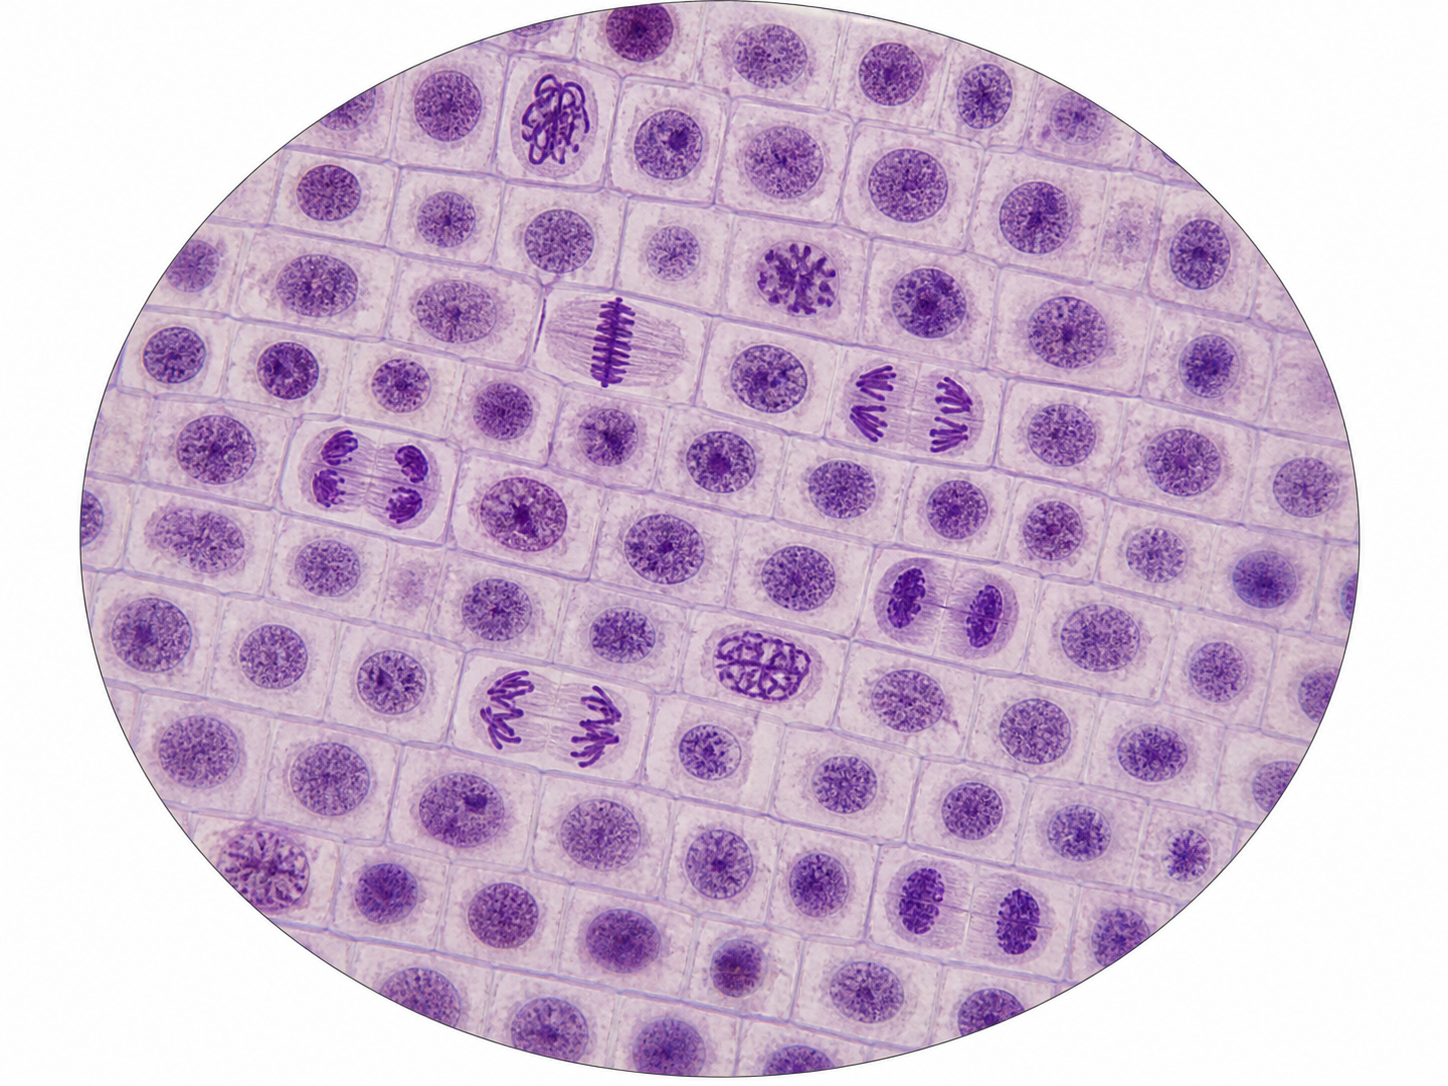
\includegraphics[width=0.58\linewidth]{images/book2/ai/g11-mitosis-root-tip.png}

{\small Preparat pencet ujung akar bawang bombai di bawah mikroskop
cahaya. Sebagian besar \omterm{def:g10:cells-common-unit:cell}{selnya} berada dalam interfase; beberapa
memperlihatkan \omterm{def:g11:cell-cycle-mitosis:chromosome}{kromosom} yang memadat pada tahap \omterm{def:g11:cell-cycle-mitosis:cycle}{mitosis} yang
berbeda-beda. Menghitung bagiannya pada tiap tahap mengukur berapa lama
tiap tahap berlangsung.}
\end{omfigure}

\begin{example}[Menghitung dalam ujung akar]\label{ex:g11:cell-cycle-mitosis:count}
Dari 600 \omterm{def:g10:cells-common-unit:cell}{sel} yang terhitung dalam sebuah ujung akar, 540 berada dalam
interfase dan 60 dalam \omterm{def:g11:cell-cycle-mitosis:cycle}{mitosis}: \emph{indeks \omterm{def:g11:cell-cycle-mitosis:cycle}{mitosis}}-nya 10\%. Jika
daurnya berlangsung 20 jam, \omterm{def:g11:cell-cycle-mitosis:cycle}{mitosisnya} berlangsung sekitar
$0.10 \times 20 = \qty{2}{h}$; dan jika 36 dari 60 \omterm{def:g10:cells-common-unit:cell}{sel} yang membelah
berada dalam profase, profasenya memakan $36/60$ dari kedua jam itu,
sekitar 72 menit, sedangkan anafasenya, yang terlihat hanya pada 4 \omterm{def:g10:cells-common-unit:cell}{sel},
memakan sekitar 8 menit. Tahap yang paling langka adalah yang paling cepat.
\end{example}

\begin{method}[Menghitung kromosom dan kromatid]\label{met:g11:cell-cycle-mitosis:counting}
Untuk \omterm{def:g10:biodiversity-scales:species}{spesies} dengan $2n$ \omterm{def:g11:cell-cycle-mitosis:chromosome}{kromosom}:
\begin{enumerate}
  \item dalam $\mathrm{G_1}$: $2n$ \omterm{def:g11:cell-cycle-mitosis:chromosome}{kromosom}, masing-masing satu
        \omterm{def:g11:cell-cycle-mitosis:chromosome}{kromatid}, \omterm{def:g10:universal-dna:information}{DNA-nya} $q$;
  \item setelah S, sepanjang $\mathrm{G_2}$, profase dan metafase: $2n$
        \omterm{def:g11:cell-cycle-mitosis:chromosome}{kromosom}, masing-masing dua \omterm{def:g11:cell-cycle-mitosis:chromosome}{kromatid} ($4n$ \omterm{def:g11:cell-cycle-mitosis:chromosome}{kromatid}), \omterm{def:g10:universal-dna:information}{DNA-nya} $2q$;
  \item sejak anafase: $4n$ \omterm{def:g11:cell-cycle-mitosis:chromosome}{kromosom} berkromatid tunggal dalam \omterm{def:g10:cells-common-unit:cell}{selnya},
        dengan $2n$ menuju tiap kutubnya;
  \item dalam tiap \omterm{def:g10:cells-common-unit:cell}{sel} anaknya: $2n$ \omterm{def:g11:cell-cycle-mitosis:chromosome}{kromosom}, masing-masing satu
        \omterm{def:g11:cell-cycle-mitosis:chromosome}{kromatid}, \omterm{def:g10:universal-dna:information}{DNA-nya} $q$.
\end{enumerate}
Sebuah \omterm{def:g11:cell-cycle-mitosis:chromosome}{kromatid} menjadi \omterm{def:g11:cell-cycle-mitosis:chromosome}{kromosom} pada saat \omterm{def:g11:cell-cycle-mitosis:chromosome}{sentromernya} membelah.
\end{method}

\begin{example}[Angka manusia]\label{ex:g11:cell-cycle-mitosis:human}
\omterm{def:g10:cells-common-unit:cell}{Sel} manusia dalam metafase memuat 46 \omterm{def:g11:cell-cycle-mitosis:chromosome}{kromosom} dan 92 \omterm{def:g11:cell-cycle-mitosis:chromosome}{kromatid}; dalam
anafase, 92 \omterm{def:g11:cell-cycle-mitosis:chromosome}{kromosom}, dengan 46 bergerak ke tiap kutubnya; tiap
anaknya, 46 \omterm{def:g11:cell-cycle-mitosis:chromosome}{kromosom} yang masing-masing satu \omterm{def:g11:cell-cycle-mitosis:chromosome}{kromatid}, yang memuat
persis \omterm{def:g10:universal-dna:information}{DNA} yang dimiliki induknya pada awal daurnya.
\end{example}

\section{Untuk apa mitosis}

\begin{proposition}[Kesesuaian dan kegunaannya]\label{prop:g11:cell-cycle-mitosis:conformity}
Karena replikasinya setia dan \omterm{def:g11:cell-cycle-mitosis:cycle}{mitosisnya} membagikan \omterm{def:g11:cell-cycle-mitosis:chromosome}{kromatidnya} dengan
tepat, setiap \omterm{def:g10:cells-common-unit:cell}{sel} tubuh bersel banyak membawa \omterm{def:g10:universal-dna:information}{informasi genetik} yang
sama dengan \omterm{def:g10:cells-common-unit:cell}{sel} telur terbuahi asalnya. \omterm{def:g11:cell-cycle-mitosis:cycle}{Mitosis} adalah mekanisme
pertumbuhan (embrio, ujung akar), pembaruan (kulit, lapisan usus,
darah: sumsum tulang sendirian membuat sekitar $\num{2e11}$ \omterm{def:g10:cells-common-unit:cell}{sel} tiap
hari) dan perbaikan (penyembuhan luka); pada eukariot bersel satu ia
adalah perkembangbiakan itu sendiri. Kendalinya --- keputusan untuk
masuk daurnya, pemeriksaan sebelum S dan sebelum anafase --- menjadi
pokok \cref{ch:g11:cancer}.
\end{proposition}
\admitted

\begin{remark}[Tidak semuanya membelah]\label{rem:g11:cell-cycle-mitosis:notall}
Sebagian besar neuron dan \omterm{def:g10:cells-common-unit:cell}{sel} otot jantung meninggalkan daurnya pada
masa kanak-kanak awal dan tidak pernah masuk lagi: kerusakan padanya
tidak diperbaiki lewat pembelahan, dan itulah sebabnya cedera tulang
belakang atau serangan jantung meninggalkan kehilangan yang menetap.
\omterm{def:g10:cells-common-unit:cell}{Sel} hati beristirahat dalam $\mathrm{G_1}$ berbulan-bulan tetapi masuk
lagi ke daurnya ketika sebagian hatinya diangkat, lalu menumbuhkan
kembali organnya dalam beberapa pekan. \omterm{def:g10:cells-common-unit:cell}{Sel} mana yang boleh membelah,
dan kapan, adalah salah satu pengaturan yang paling ketat dalam tubuh.
\end{remark}

\section{Latihan}

\begin{exercise}[$\star$]\label{exo:g11:cell-cycle-mitosis:1}
Sebutkan keempat fase \omterm{def:g11:cell-cycle-mitosis:cycle}{daur sel} dan sebutkan apa yang terjadi pada masing-masing.
\end{exercise}

\begin{exercise}[$\star$]\label{exo:g11:cell-cycle-mitosis:2}
Rumuskan \omterm{def:g11:cell-cycle-mitosis:chromosome}{kromatid} dan \omterm{def:g11:cell-cycle-mitosis:chromosome}{sentromer}. Kapan sebuah \omterm{def:g11:cell-cycle-mitosis:chromosome}{kromosom} punya dua
\omterm{def:g11:cell-cycle-mitosis:chromosome}{kromatid}?
\end{exercise}

\begin{exercise}[$\star$]\label{exo:g11:cell-cycle-mitosis:3}
Sebutkan keempat tahap \omterm{def:g11:cell-cycle-mitosis:cycle}{mitosis} beserta satu peristiwa pentingnya.
\end{exercise}

\begin{exercise}[$\star$]\label{exo:g11:cell-cycle-mitosis:4}
Sebuah \omterm{def:g10:cells-common-unit:organelle}{inti sel} memuat \omterm{def:g10:universal-dna:information}{DNA} sebanyak $1.5q$. \omterm{def:g10:cells-common-unit:cell}{Sel} itu berada dalam fase apa?
\end{exercise}

\begin{exercise}[$\star$]\label{exo:g11:cell-cycle-mitosis:5}
Berapa banyak \omterm{def:g11:cell-cycle-mitosis:chromosome}{kromosom}, dan berapa banyak \omterm{def:g11:cell-cycle-mitosis:chromosome}{kromatid}, yang dimiliki \omterm{def:g10:cells-common-unit:cell}{sel}
manusia dalam $\mathrm{G_2}$?
\end{exercise}

\begin{exercise}[$\star\star$]\label{exo:g11:cell-cycle-mitosis:6}
Dari gambar jumlah \omterm{def:g10:universal-dna:information}{DNA-nya}, sebutkan lama tiap fasenya dan sebutkan
dalam fase mana saja sebuah \omterm{def:g10:cells-common-unit:cell}{sel} akan ditemukan dengan $2q$.
\end{exercise}

\begin{exercise}[$\star\star$]\label{exo:g11:cell-cycle-mitosis:7}
Seekor mencit punya $2n = 40$. Sebutkan jumlah \omterm{def:g11:cell-cycle-mitosis:chromosome}{kromosom} dan jumlah
\omterm{def:g11:cell-cycle-mitosis:chromosome}{kromatid} dalam \omterm{def:g10:cells-common-unit:cell}{sel} pada metafase, pada anafase (seluruh \omterm{def:g10:cells-common-unit:cell}{selnya}), dan
dalam sebuah \omterm{def:g10:cells-common-unit:cell}{sel} anaknya.
\end{exercise}

\begin{exercise}[$\star\star$]\label{exo:g11:cell-cycle-mitosis:8}
Dalam sebuah ujung akar, 800 \omterm{def:g10:cells-common-unit:cell}{sel} terhitung: 720 dalam interfase, 48
dalam profase, 16 dalam metafase, 6 dalam anafase, 10 dalam telofase.
Hitung indeks \omterm{def:g11:cell-cycle-mitosis:cycle}{mitosisnya} dan, untuk daur 24 jam, lama tiap tahapnya.
\end{exercise}

\begin{exercise}[$\star\star$]\label{exo:g11:cell-cycle-mitosis:9}
Kolkisin, obat yang disari dari krokus musim gugur, mencegah
gelendongnya terbentuk. Ramalkan apa yang terjadi pada \omterm{def:g10:cells-common-unit:cell}{sel} yang membelah
yang diperlakukan dengannya, dan mengapa ahli biologi memakainya untuk
menyiapkan \omterm{def:g11:cell-cycle-mitosis:chromosome}{kariotipe}.
\end{exercise}

\begin{exercise}[$\star\star$]\label{exo:g11:cell-cycle-mitosis:10}
Jelaskan mengapa \omterm{def:g11:cell-cycle-mitosis:chromosome}{kromosomnya} harus memadat sebelum dipindahkan, dan
mengapa \omterm{def:g11:cell-cycle-mitosis:chromosome}{kromosomnya} terurai lagi sesudahnya.
\end{exercise}

\begin{exercise}[$\star\star$]\label{exo:g11:cell-cycle-mitosis:11}
\omterm{def:g10:cells-common-unit:cell}{Sel} telur yang terbuahi membelah tiap 12 jam pada hari-hari pertamanya.
Ada berapa \omterm{def:g10:cells-common-unit:cell}{sel} setelah 5 hari? Apakah tiap pembelahan akan memerlukan
$\mathrm{G_1}$ yang penuh?
\end{exercise}

\begin{exercise}[$\star\star\star$]\label{exo:g11:cell-cycle-mitosis:12}
Pada anafase kedua \omterm{def:g11:cell-cycle-mitosis:chromosome}{kromatid} satu \omterm{def:g11:cell-cycle-mitosis:chromosome}{kromosom} gagal memisah dan keduanya
pergi ke kutub yang sama. Lukiskan kedua \omterm{def:g10:cells-common-unit:cell}{sel} anaknya (jumlah \omterm{def:g11:cell-cycle-mitosis:chromosome}{kromosom},
\omterm{def:g10:universal-dna:information}{DNA}) dan jelaskan mengapa kesalahan semacam itu, dalam \omterm{def:g10:cells-common-unit:cell}{sel} tubuh,
lazimnya tanpa akibat tetapi dalam beberapa hal serius.
\end{exercise}

\begin{exercise}[$\star\star\star$]\label{exo:g11:cell-cycle-mitosis:13}
Sumsum tulang membuat $\num{2e11}$ \omterm{def:g10:cells-common-unit:cell}{sel} darah tiap hari. Jika \omterm{def:g10:cells-common-unit:cell}{sel} bakal
sumsum berdaur dalam 24 jam, perkirakan berapa banyak \omterm{def:g10:cells-common-unit:cell}{sel} bakal yang
sedang membelah pada suatu saat, dan beri tanggapan atas apa yang akan
diperbuat obat penghalang \omterm{def:g11:cell-cycle-mitosis:cycle}{mitosis} pada darahnya dalam sepekan.
\end{exercise}

\begin{exercise}[$\star\star\star$]\label{exo:g11:cell-cycle-mitosis:14}
Jelaskan mengapa \omterm{def:g11:cell-cycle-mitosis:chromosome}{kariotipe} disiapkan dari \omterm{def:g10:cells-common-unit:cell}{sel} yang ditahan pada
metafase alih-alih pada interfase atau anafase.
\end{exercise}

\begin{exercise}[$\star\star\star$]\label{exo:g11:cell-cycle-mitosis:15}
Sebuah hati diangkat dua pertiganya; dalam tiga pekan ia telah tumbuh
kembali. Dengan \omterm{def:g11:cell-cycle-mitosis:cycle}{daur selnya}, lukiskan apa yang diperbuat \omterm{def:g10:cells-common-unit:cell}{selnya}, dan
sebutkan seperti apa kandungan \omterm{def:g10:universal-dna:information}{DNA} \omterm{def:g10:cells-common-unit:cell}{sel} hatinya pada hari ke-3
dibandingkan hari ke-0.
\end{exercise}

\section{Soal: Jadwal Ujung Akar}

\begin{problem}[{Soal akhir pekan --- sebuah ujung akar yang dihitung
sel demi sel: lama tiap tahap daurnya, DNA pada tiap saat, sel yang
dibuat sebuah akar dalam sehari, dan delapan menit anafasenya}]
\label{pb:g11:cell-cycle-mitosis:1}
Sebuah kelas mencetak dan mewarnai ujung akar bawang putih ($2n = 16$)
lalu menghitung 1000 \omterm{def:g10:cells-common-unit:cell}{sel} dalam zona pertumbuhannya: 900 dalam
interfase, 60 dalam profase, 18 dalam metafase, 8 dalam anafase, 14
dalam telofase. Pengukuran yang mandiri memberi \omterm{def:g11:cell-cycle-mitosis:cycle}{daur sel} itu 20 jam.
Ambil zona pertumbuhannya memuat 20\,000 \omterm{def:g10:cells-common-unit:cell}{sel}.

\medskip
\noindent\textbf{Bagian I --- Indeks \omterm{def:g11:cell-cycle-mitosis:cycle}{mitosisnya}.}
\begin{enumerate}
  \item Hitung indeks \omterm{def:g11:cell-cycle-mitosis:cycle}{mitosis} jaringannya.
  \item Dengan menganggap bahwa bagian \omterm{def:g10:cells-common-unit:cell}{sel} dalam sebuah tahap sama
        dengan bagian daur yang dihabiskan di dalamnya, hitung lama
        \omterm{def:g11:cell-cycle-mitosis:cycle}{mitosisnya}.
  \item Hitung lama masing-masing keempat tahapnya.
  \item Tahap mana yang terpendek? Usulkan mengapa ia dapat secepat itu.
  \item Mengapa caranya menuntut penghitungan banyak \omterm{def:g10:cells-common-unit:cell}{sel}, dan mengapa
        \omterm{def:g10:cells-common-unit:cell}{selnya} harus berasal dari zona pertumbuhannya saja?
\end{enumerate}

\medskip
\noindent\textbf{Bagian II --- \omterm{def:g11:cell-cycle-mitosis:chromosome}{Kromosom} dan \omterm{def:g10:universal-dna:information}{DNA-nya}.}
\begin{enumerate}[resume]
  \item Berapa banyak \omterm{def:g11:cell-cycle-mitosis:chromosome}{kromosom}, dan berapa banyak \omterm{def:g11:cell-cycle-mitosis:chromosome}{kromatid}, yang dimuat
        \omterm{def:g10:cells-common-unit:cell}{sel} bawang putih pada metafase?
  \item Berapa banyak \omterm{def:g11:cell-cycle-mitosis:chromosome}{kromosom} yang bergerak dalam \omterm{def:g10:cells-common-unit:cell}{sel} anafase, dan
        berapa banyak yang mencapai tiap kutubnya?
  \item Dengan menyebut $q$ \omterm{def:g10:universal-dna:information}{DNA} sebuah \omterm{def:g10:cells-common-unit:cell}{sel} anak, sebutkan kandungan \omterm{def:g10:universal-dna:information}{DNA}
        \omterm{def:g10:cells-common-unit:cell}{sel} dalam profase, dalam anafase (seluruh \omterm{def:g10:cells-common-unit:cell}{selnya}) dan dalam
        telofase (tiap \omterm{def:g10:cells-common-unit:organelle}{inti selnya}).
  \item Dari 900 \omterm{def:g10:cells-common-unit:cell}{sel} interfasenya, kira-kira berapa yang berada dalam
        S, jika $\mathrm{G_1}$, S dan $\mathrm{G_2}$ memakan 8, 7 dan 4 jam?
  \item Seorang murid menemukan \omterm{def:g10:cells-common-unit:cell}{sel} dengan 32 \omterm{def:g11:cell-cycle-mitosis:chromosome}{kromosom} berkromatid
        tunggal yang tersebar dalam \omterm{def:g10:cells-common-unit:cell}{sitoplasmanya}. Tahap apa itu, dan
        apa yang baru saja terjadi?
\end{enumerate}

\medskip
\noindent\textbf{Bagian III --- Keluaran akarnya.}
\begin{enumerate}[resume]
  \item Jika tiap \omterm{def:g10:cells-common-unit:cell}{sel} zona pertumbuhannya berdaur dalam 20 jam, berapa
        banyak \omterm{def:g10:cells-common-unit:cell}{sel} baru yang dihasilkan zona itu tiap jam?
  \item Tiap \omterm{def:g10:cells-common-unit:cell}{sel} baru, begitu keluar dari zona pertumbuhannya,
        memanjang sampai sekitar \qty{100}{\micro m}. Dalam sederet \omterm{def:g10:cells-common-unit:cell}{sel}
        selebar satu \omterm{def:g10:cells-common-unit:cell}{sel}, berapa panjang akarnya bertambah tiap hari?
        Bandingkan dengan \qty{1}{mm} sehari yang teramati dan jelaskan bedanya.
  \item Tiap \omterm{def:g10:cells-common-unit:cell}{sel} anaknya harus menyalin $2n = 16$ \omterm{def:g11:cell-cycle-mitosis:chromosome}{kromosom}, sekitar
        $\num{1.6e10}$ pasangan \omterm{def:g10:universal-dna:nucleotide}{basa} seluruhnya. Dengan garpu 50
        \omterm{def:g10:universal-dna:nucleotide}{nukleotida} tiap sekon, berapa titik awal yang diperlukan untuk
        selesai dalam 7 jam fase S-nya?
  \item Akarnya ditaruh dalam dingin (\qty{4}{\celsius}) selama sehari.
        Ramalkan perubahan hitungannya, dan perubahan indeks \omterm{def:g11:cell-cycle-mitosis:cycle}{mitosisnya}
        jika dingin memperlambat semua fasenya sama rata.
  \item Sebuah herbisida menghalangi \omterm{prop:g11:dna-replication:forks}{DNA polimerase}. Setelah sehari,
        tahap mana yang masih akan terlihat dalam preparatnya, dan mana
        yang akan lenyap? Jelaskan.
\end{enumerate}

\medskip
\noindent\textbf{Bagian IV --- Putusan hitungannya.}
\begin{enumerate}[resume]
  \item Kelas kedua menghitung jaringan yang sama dan menemukan 4
        anafase dalam 1000 \omterm{def:g10:cells-common-unit:cell}{sel}. Lama apa yang mereka hitung? Apakah
        ketidaksepakatannya mengejutkan bagi tahap yang terlihat pada
        segelintir \omterm{def:g10:cells-common-unit:cell}{sel}?
  \item Dengan menggabungkan kedua kelasnya (2000 \omterm{def:g10:cells-common-unit:cell}{sel}, 12 anafase),
        hitung ulang lama anafasenya.
  \item \omterm{def:g10:cells-common-unit:cell}{Sel} manusia dalam biakan punya indeks \omterm{def:g11:cell-cycle-mitosis:cycle}{mitosis} 4\% dan daur 24
        jam. Bandingkan lama \omterm{def:g11:cell-cycle-mitosis:cycle}{mitosisnya} dengan lama \omterm{def:g11:cell-cycle-mitosis:cycle}{mitosis} bawang putihnya.
  \item Jelaskan mengapa indeks \omterm{def:g11:cell-cycle-mitosis:cycle}{mitosis} sebuah tumor sering beberapa
        kali indeks jaringan asalnya, dan apa maknanya bagi obat yang
        bekerja pada gelendongnya.
  \item Nyatakan hasilnya: jadwal \omterm{def:g11:cell-cycle-mitosis:cycle}{daur sel} akar bawang putih, tahap
        demi tahap, dan tahap yang delapan menitnya memutuskan bahwa
        tiap anaknya memperoleh enam belas \omterm{def:g11:cell-cycle-mitosis:chromosome}{kromosom}.
\end{enumerate}
\end{problem}
